% TeX encoding = utf8
% TeX spellcheck = pl_PL 
\documentclass[a4paper, 11pt]{article}
\usepackage[utf8]{inputenc}
\usepackage[polish]{babel}
\usepackage{polski}
\usepackage{float}
\usepackage{graphicx}
\usepackage{listings}
\usepackage{amsfonts}
\usepackage{geometry}
\usepackage{multicol}
\usepackage{latexsym}
\usepackage{enumerate}
\usepackage{hyperref}
\usepackage{wrapfig}
\usepackage{color} %red, green, blue, yellow, cyan, magenta, black, white
\definecolor{mygreen}{RGB}{28,172,0} % color values Red, Green, Blue
\definecolor{mylilas}{RGB}{170,55,241}

\author{Kamil Foryszewski}
\title{Sterowanie Procesami - projekt 2, zadanie 2.16}
\frenchspacing

\newgeometry{tmargin=2cm, bmargin=2cm, lmargin=2cm, rmargin=2cm}
\pagestyle{empty}


\begin{document}

\lstset{language=Matlab,%
    basicstyle=\color{red},
    breaklines=true,%
    morekeywords={matlab2tikz},
    keywordstyle=\color{blue},%
    morekeywords=[2]{1}, keywordstyle=[2]{\color{black}},
    identifierstyle=\color{black},%
    stringstyle=\color{mylilas},%
    commentstyle=\color{mygreen},%
    showstringspaces=false,
    numbers=right,%
    numberstyle={ \color{black}},% size of the numbers
    numbersep=5pt, % this defines how far the numbers are from the text
    emph=[1]{for,endfor,endwhile,endfunction,endif,break},emphstyle=[1]\color{blue}, %some words to emphasise
    emph=[2]{,.}, emphstyle=[2]\color{yellow},%
}

\maketitle
\tableofcontents

\section{Polecenie}
Obiekt regulacji jest opisany transmitancją: 
$$G(s) = \frac{K_0e^{-T_0s}}{(T_1s + 1)(T_2s+1)}  = \frac{3.5e^{-T_0s}}{10.04s^2+7.02s +1}  $$
Gdzie: 
$K_0 = 3.5, T_0 = 5, T_1 = 2, T_2 = 5.02$

\section{Transmitancja dyskretna}
Wyznaczona transmitancja dyskretna ma następującą postać: 
$$G(z) = z^{-10}\frac{0.0388z+0.0346}{z^2-1.684z+0.705}$$
Została wyznaczona przy pomocy polecenia \emph{c2d} pakietu matlab. 
\begin{figure}[H]
\centering
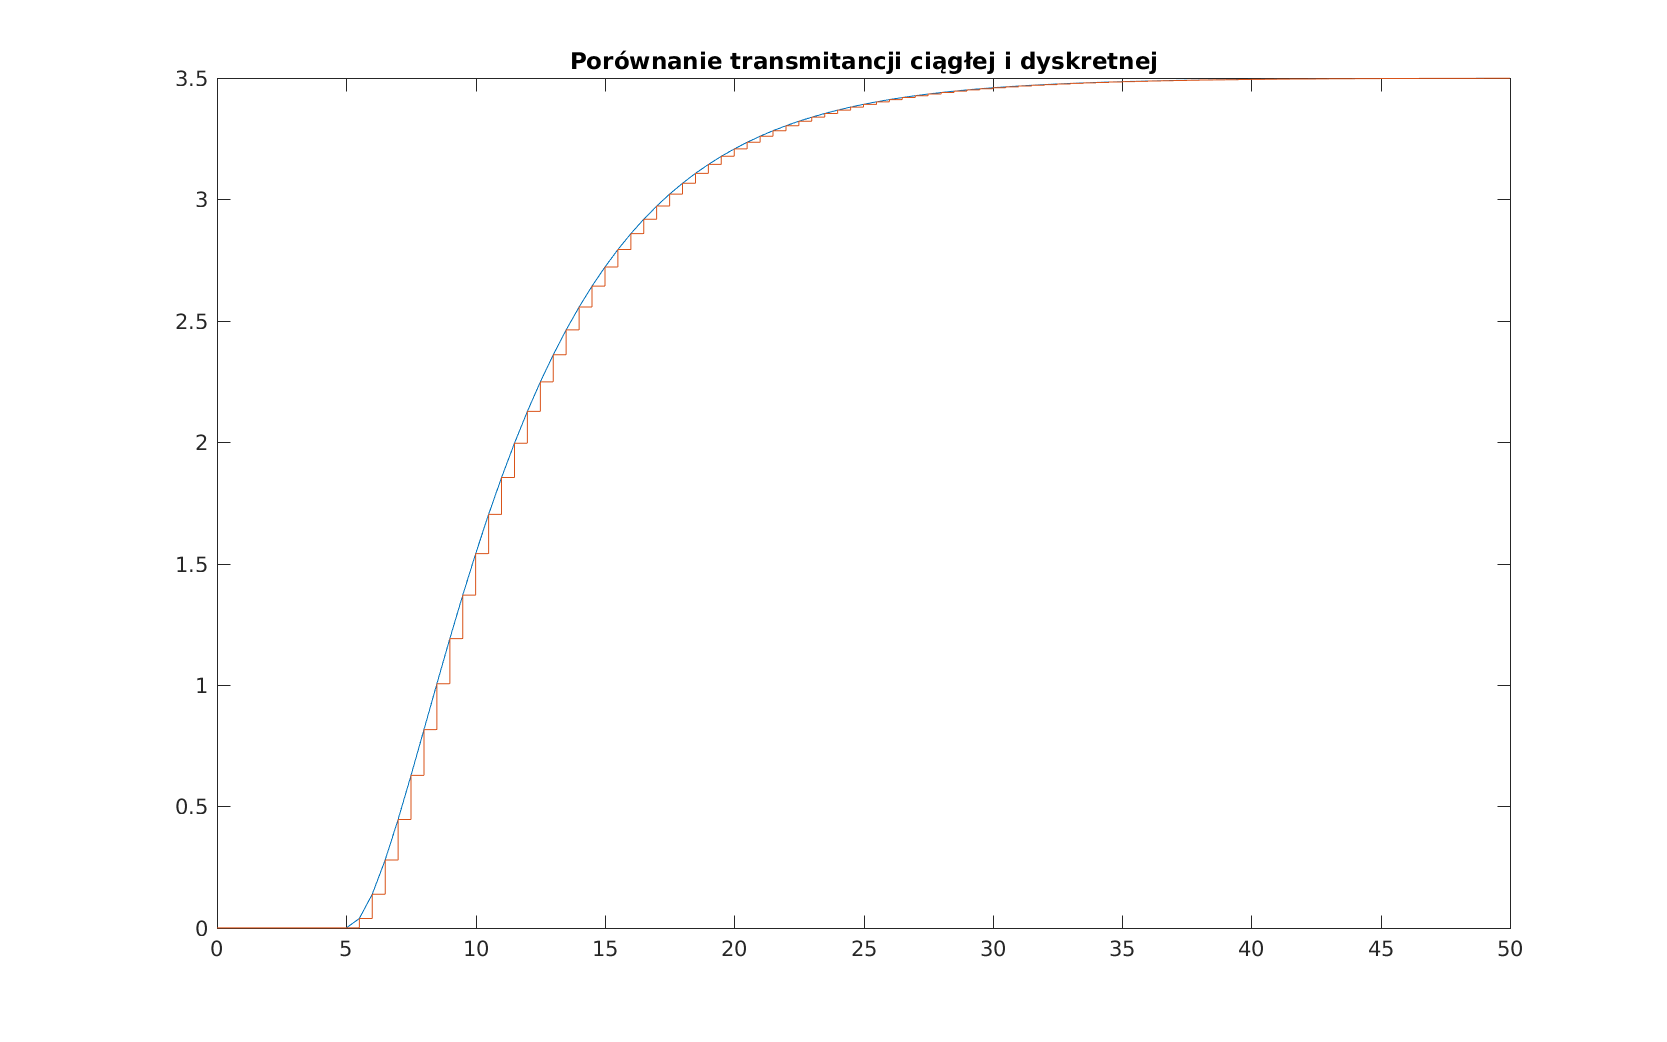
\includegraphics[scale=0.6]{1_1.png}
\caption{Odpowiedź skokowa transmitancji ciągłej i dyskretnej}
\label{step:1}
\end{figure}
Odpowiedź skokowa obu transmitancji w przybliżeniu jest taka sama. Odpowiedzi skokowe obliczone jako granice transmitancji przy argumentach $s$ dążącym do $0$ i $z$ dążącym do $1$ są również bardzo zbliżone. Wzmocnienie statyczne transmitancji ciągłej $K_c = 5$, natomiast wzmocnienie statyczne transmitancji dyskretnej $K_d = 5.0572$

\section{Równanie różnicowe}
Korzystając z transmitancji możemy wyznaczyć równanie różnicowe opisujące obiekt w postaci: 

$$y(k) = \sum_{i=1}^{n} b_iy(k-i)+ \sum_{i=1}^{m} c_iu(k-1)$$
Należy zatem przekształcić transmitancję do następującej postaci: 
$$G(z) = \frac{0.0388z^{-11}+0.0346z^{-12}}{z-1.684z^{-1}+0.705z^{-2}} = \frac{Y(z)}{U(z)}$$
Po przekształceniu: 
$$Y(z)(1-1.6840z^{-1}+0.7050z^{-2}) = U(z)(0.0388z^{-11}+0.0346z^{-12})$$
Skąd możemy bezpośrednio przejść do równania różnicowego: 
\begin{equation}\
\label{rozn}
y(k) = 1.684y(k-1) - 0.705y(k-2) + 0.0388u(k-11) + 0.0346u(k-12)
\end{equation}


\section{Dobór regulatora PID metodą Zieglera-Nicholsa}
Transmitancja ciągłego regulatora PID wygląda następująco: 
$$R(s) = k_r(1=\frac{1}{T_is}+T_ds)=K_p + K_i\frac{1}{s}+K_ds$$
Pierwszym etapem metody Zieglera-Nicholsa jest wyznaczenie wzmocnienia krytycznego $K$, dla którego sygnał wyjściowy utrzymuje się na poziomie oscylacji, wokół wartości zadanej, ze stałą amplitudą. Przy parametrach $K_i, K_d=0$ stopniowo zwiększamy wartość parametru $K_p$ aż do wystąpienia oscylacji niegasnących o stałej amplitudzie. Dla tak wyznaczonego wzmocnienia odczytujemy również okres oscylacji $T_{osc}$. Wyznaczone parametry wynoszą: \\

$K_{kr} = 0.6314$\\
\indent $T_{osc} = 17$\\

Posiadając wzmocnienie krytyczne i okres oscylacji możemy obliczyć pozostałe parametry na podstawie tabelki: 
\begin{table}[htp]
\centering
\caption{Tabela nastaw PID}
\begin{tabular}{|l|l|l|l|}
\hline
    & $K_p$       & $K_i $                & $K_d $              \\
\hline
P   & $0.5K_{kr} $ &                    &                   \\
\hline
PI   & $0.45K_{kr}$ & $\frac{1.2K_p}{T_{osc}}$ &                   \\
\hline
PID & $0.6K_{kr} $ & $\frac{2K_p}{T_{osc}}$   & $\frac{8K_p}{T_{osc}}$ \\
\hline
\end{tabular}
\end{table}
Wynoszą one :\\

$K_p = 0.37884$\\
\indent$K_i = 0.03714$\\
\indent$K_d = 0.14856$\\
\\

\begin{figure}[H]
\centering
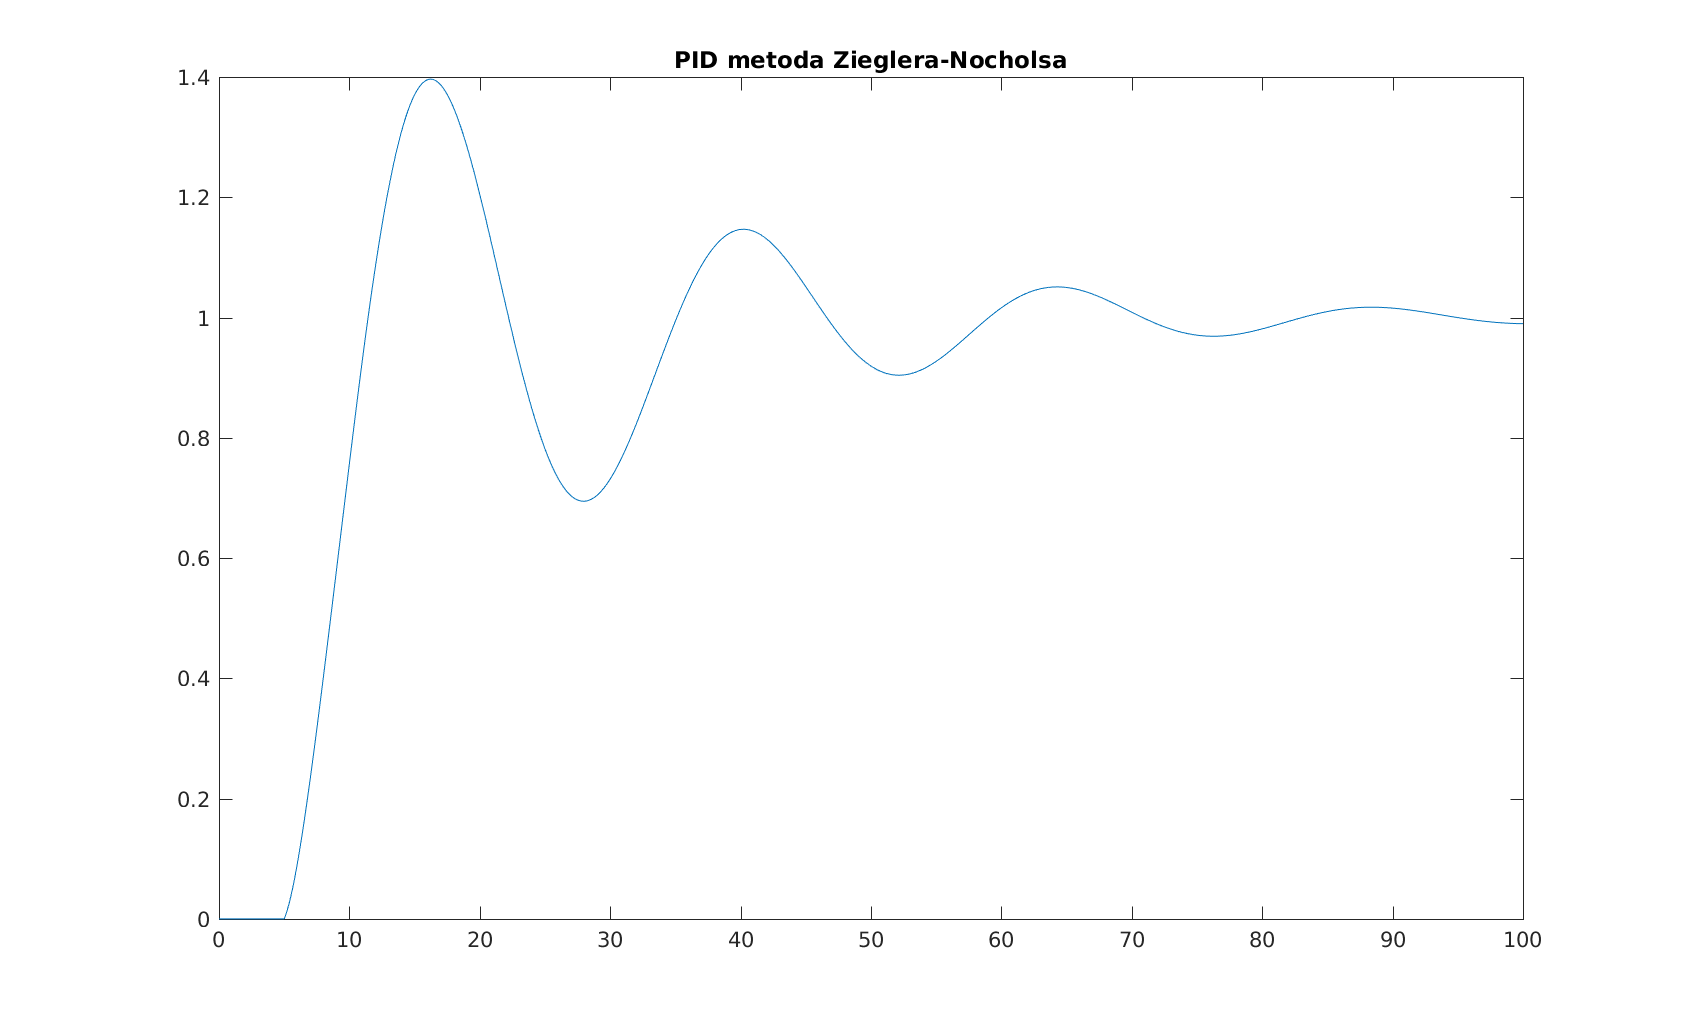
\includegraphics[scale=0.60]{2_1.png}
\caption{Odpowiedź układu na skok jednostkowy z wybranymi parametrami}
\end{figure}


\noindent Wyznaczone metodą Zieglera-Nicholsa parametry nie zapewniły dostatecznie dobrej regulacji, w celu poprawy zostało delikatnie zmniejszone wzmocnienie regulatora oraz kilkukrotnie zwiększono stałą różniczkowania, co zapewniło następujące rezultaty: \\

$K_p = 0.35$\\
\indent$K_i = 0.035$\\
\indent$K_d = 0.7$\\
\\

\begin{figure}[H]
\centering
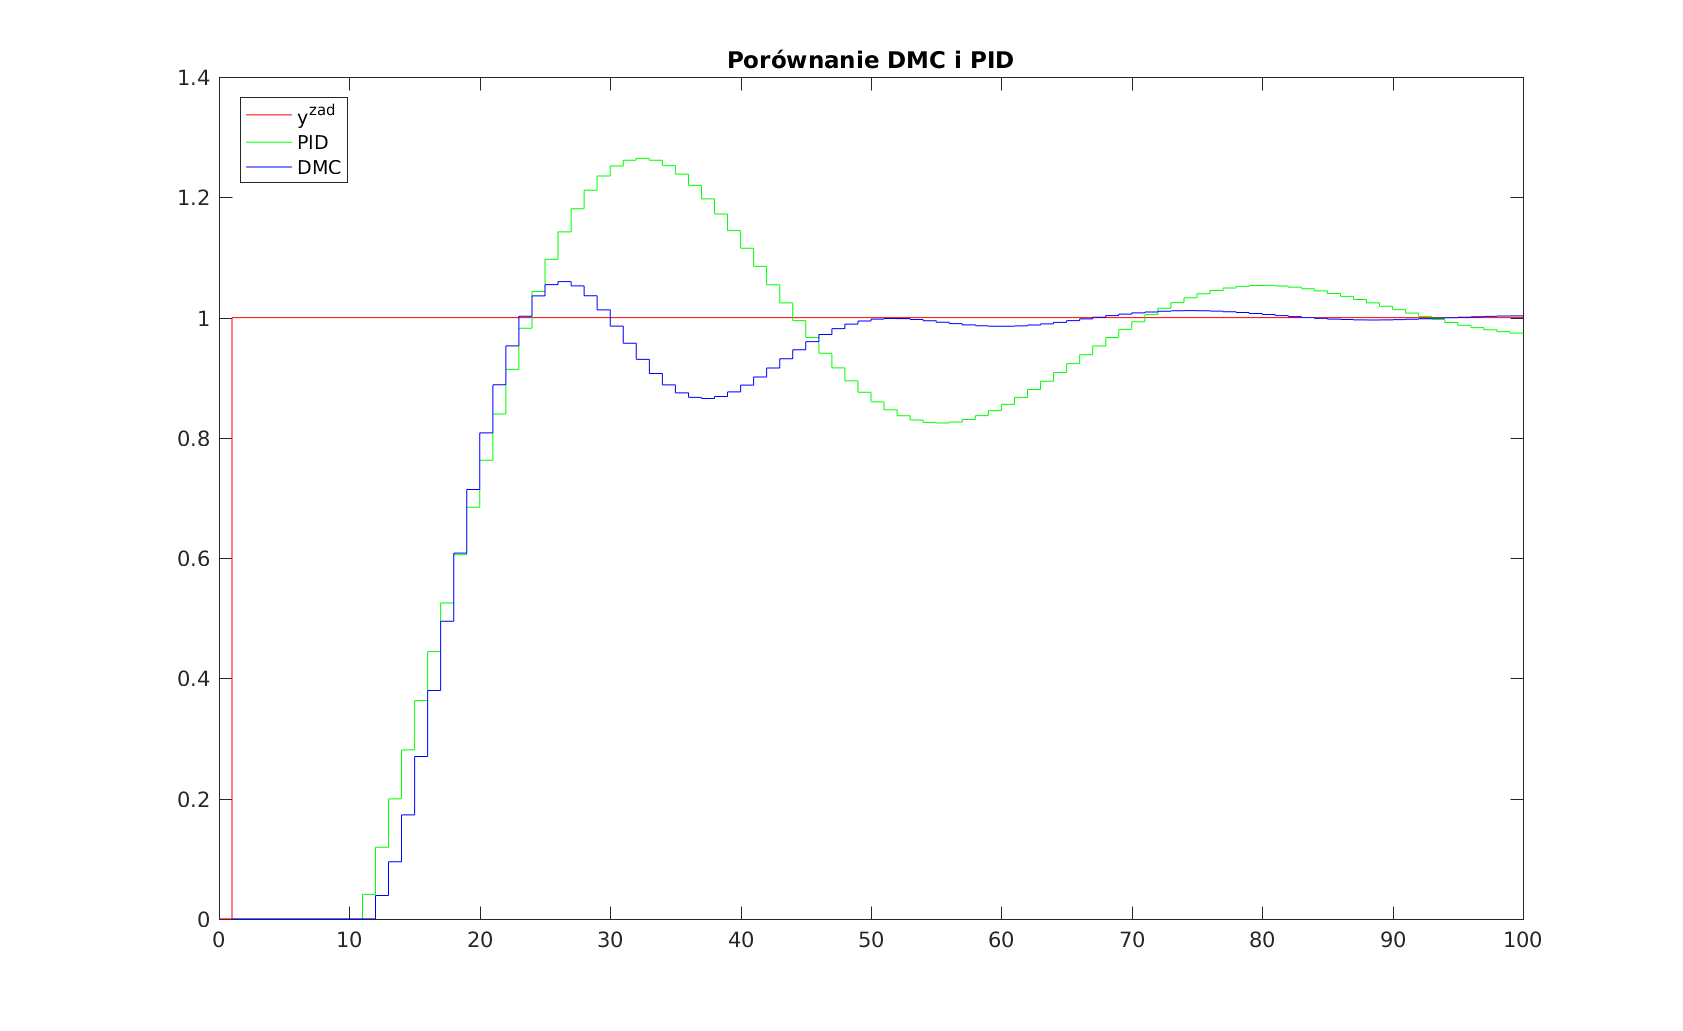
\includegraphics[scale=0.60]{2_1_1.png}
\caption{Odpowiedź układu na skok jednostkowy z dostrojonymi parametrami}
\end{figure}

\subsection{Dyskretny regulator PID}
Transmitancja dyskretnego regulatora PID ma następującą postać: 
$$R(z) = \frac{r_2z^{-2} + r_1z^{-1} + r_0}{1-z^{-1}}$$
Korzystając z przekształcenia transformaty $Z$ otrzymujemy następujące równanie: 
$$R(z) = \frac{(K_p+K_d)+(K_iT_p-K_p-2K_d)z^{-1} + K_dz^{-2}}{1-z^{-1}}$$
Porównując z ogólną postacią transmitancji dyskretnej otrzymujemy wartości parametrów: \\

$r_2 = K_d$\\
\indent$r_1 = K_iT_p -K_p-2K_d$\\
\indent$r_0 = K_p + K_d$\\

\noindent Co po podstawieniu wyznaczonych nastaw daje: \\

$r_2 = 0.14856$\\ 
\indent $r_1 = -0.672246$\\
\indent $r_0 = 0.5274$\\

Okres próbkowania $T_p$ wynosi $0.5s$

\begin{figure}[htp]
\centering
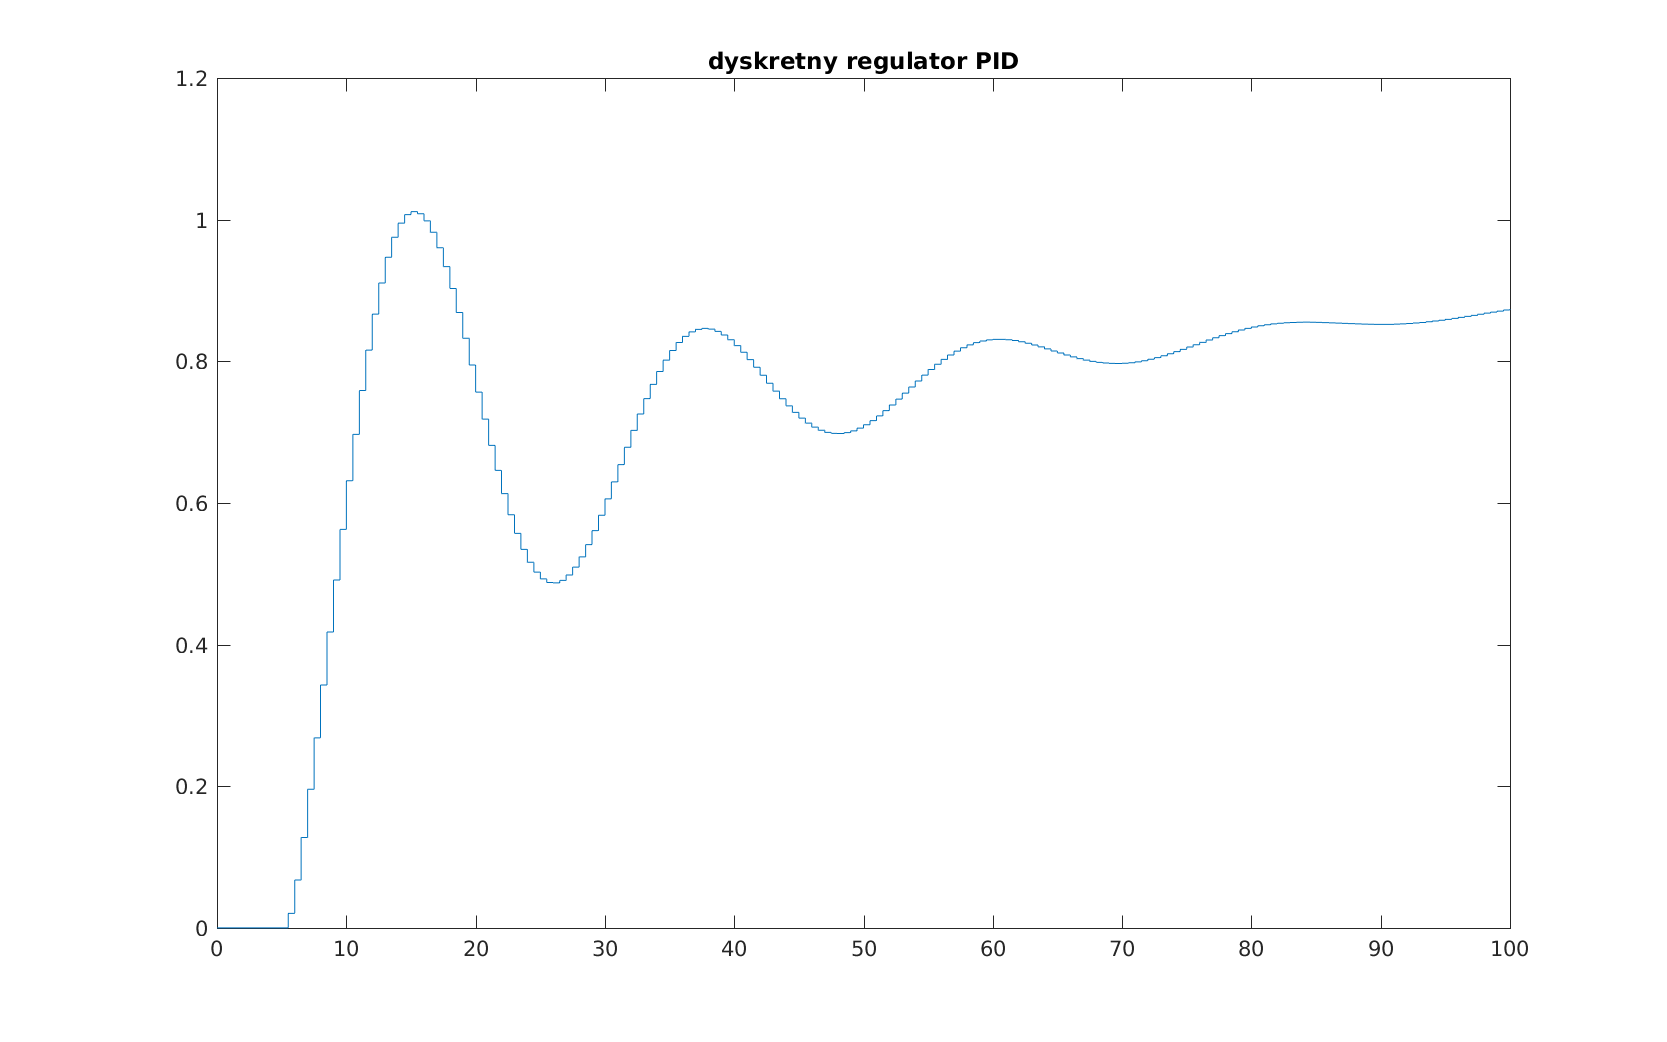
\includegraphics[scale=0.60]{2_2.png}
\caption{Odpowiedź układu na skok jednostkowy w przypadku regulatora dyskretnego}
\end{figure}

\section{Symulacja cyfrowego algorytmu PID oraz DMC }
\subsection{Symulacja dyskretnego algorytmu PID}
Implementacja symulacji dyskretnego algorytmu PID znajduje się w pliku \textbf{PID.m}. Skrypt został wykorzystany w poprzednim podpunkcie. 
\subsection{Symulacja algorytmu DMC w wersji analitycznej}
 Rozwiązanie analityczne algorytmu regulacji DMC(Dynamic Matrix Control) ma następującą postać: 
 $$\Delta u = (M^TM+\lambda I)^-1M^t(y^{zad}-y^k-M^p\Delta u^p) $$
Parametry algorytmu wyznaczamy z odpowiedzi skokowej rys:~\ref{step:1}, skorzystamy w tym celu z równania \ref{rozn} modelu wyznaczonego w podpunkcie 3. Z wartości odpowiedzi skokowej układu w poszczególnych chwilach czasu wyznaczamy macierz $M$ oraz $M^p$. Wartość sygnału wyjściowego opisuje równanie: 
$$y = y^0 + M\Delta u = y^k +M^P \Delta u^P + M\Delta u$$
Skrypt pakietu matlab znajduje się w pliku \textbf{DMC.m}. Są w nim zdefiniowane niezbędne parametry algorytmu takie jak: horyzont predykcji, horyzont dynamiki, horyzont sterowania oraz wskaźnik jakości $\lambda$. 
\section{Dobór parametrów algorytmu DMC}

\subsection{Parametry początkowe}
Horyzont dynamiki określamy na podstawie odpowiedzi skokowej rys:~\ref{step:1} i jest on numerem iteracji w której następuje ustalenie się sygnału odpowiedzi skokowej. W przypadku zadania jest to 40-sta sekunda symulacji czyli 80-ty krok symulacji, ponieważ okres próbkowania wynosi pół sekundy. Przyjmując taki horyzont predykcji otrzymujemy: 
$D = N = N_u = 80$
Jako wartość parametru $\lambda$ przyjmujemy 1, aby nie wpływał on znacząco na symulację. 
\begin{figure}[H]
\centering
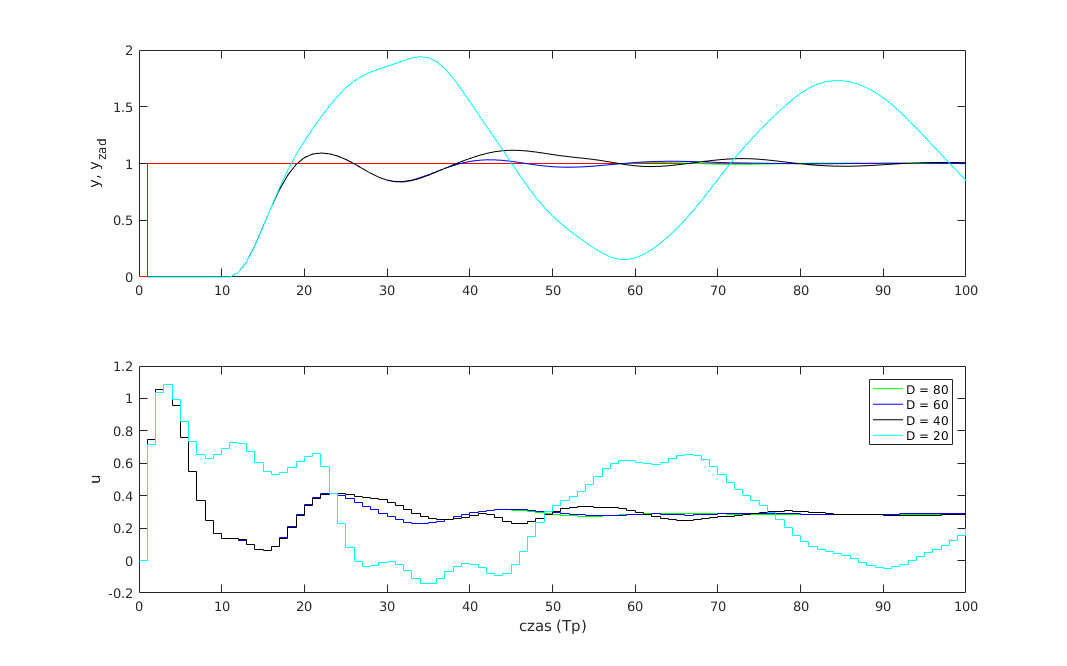
\includegraphics[scale=0.60]{horyzont_predykcji_dmc.png}
\caption{Sterowanie dla wyznaczonego horyzontu predykcji}
\end{figure}

\subsection{Skracanie horyzontu predykcji}
Najmniejsza wartość horyzontu predykcji dla której nie następuje pogorszenie regulacji wynosi 60. Poniżej wykres dla kilku wartości horyzontu predykcji. 
\begin{figure}[H]
\centering
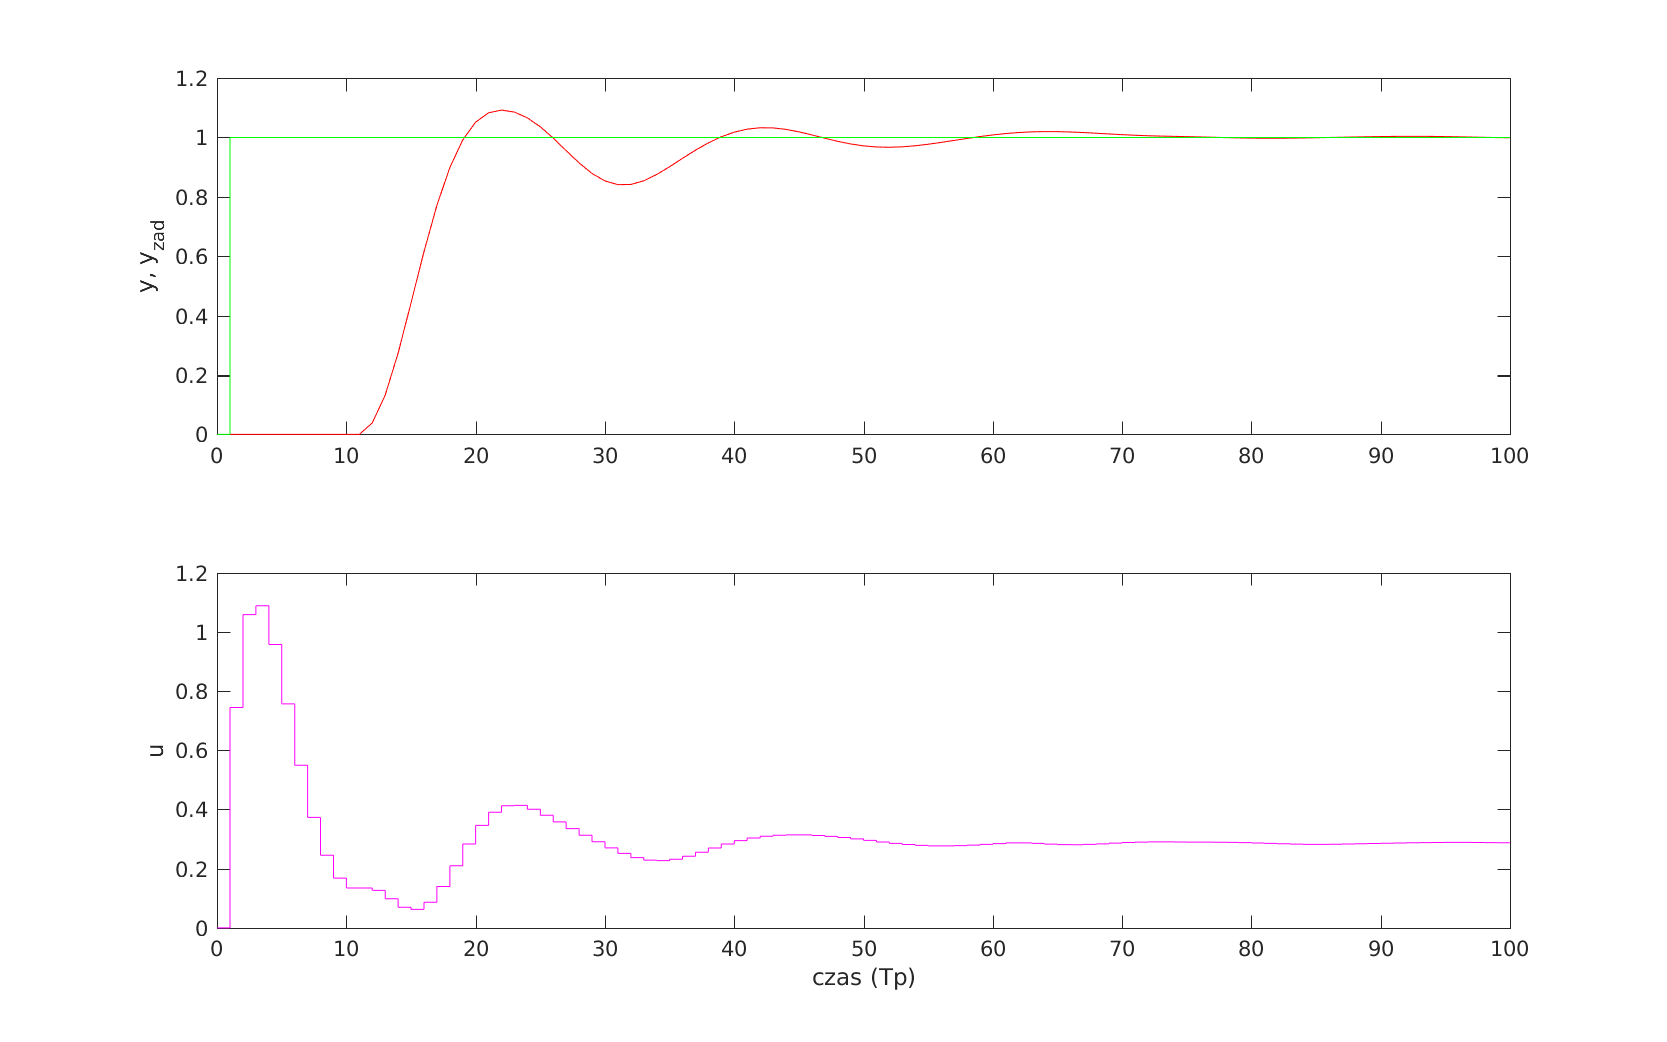
\includegraphics[scale=0.60]{horyzont_predykcji_skracanie.png}
\caption{Zmniejszony horyzont predykcji}
\end{figure}

\subsection{Wpływ długości horyzontu sterowania}
Symulując algorytm regulacji dla różnych wartości horyzontu sterowania, począwszy od wartości 1, i obserwując jakoś sterowania, wartość została określona jako 7, poniżej zeswatanie kilku symulacji o różnych wartościach współczynnika. Dla większych wartości nie następuje znaczna poprawa a wręcz pogorszenie, natomiast dla mniejszych wartości, czas regulacji zaczyna się wydłużać. 
\begin{figure}[H]
\centering
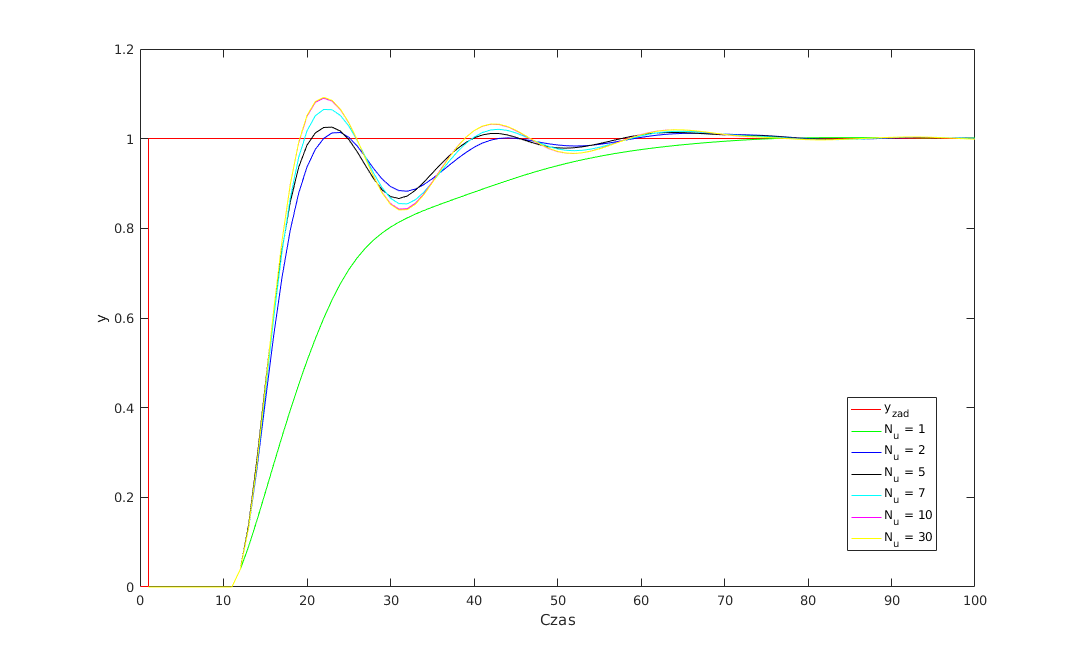
\includegraphics[scale=0.60]{horyzont_sterowania.png}
\caption{Zestawienie regulacji dla różnych wartości horyzontu sterowania}

\end{figure}

\subsection{Parametr kary $\lambda$}
Współczynnik $\lambda$ jest wskaźnikiem jakości regulacji i pełni funkcję kary za przeregulowanie. Im większa jego wartość tym łagodniej będzie się zmieniał sygnał sterujący. Poniżej kilka wykresów dla różnych parametrów $\lambda$. Dla początkowej wartości równej 1, obserwujemy gwałtowny skok sterowania który może być niedopuszczalny w wielu rzeczywistych systemach regulacji. Wartość współczynnika która zapewnia stosunkowo łagodny przebieg sygnału sterującego oraz akceptowalny czas regulacji jest $\lambda = 10$

\begin{figure}[H]
\centering
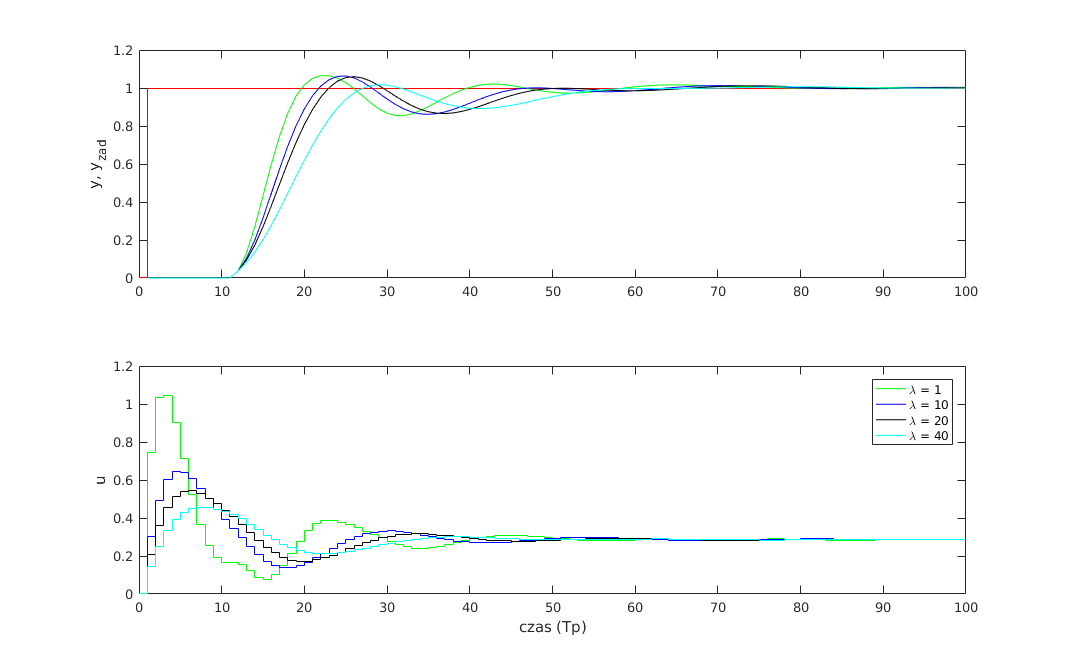
\includegraphics[scale=0.60]{lambda_dmc.png}
\caption{Wykres dla różnych wartości współczynnika kary}
\end{figure}
\subsection{Parametry dostrojonego regulatora DMC}

Ostatecznie wybrane nastawy regulatora DMC:\\

horyzont predykcji: $N = 60$\\

horyzont dynamiki: $D = 60$\\

horyzont sterowania: $N_u = 7$\\

wzkaźnik jakości: $\lambda = 10$\\

\noindent Programy wykorzystane do obliczeń fdmc.m, ddmc.m, oraz do generowania wykresów: DMCwykresy.m\\


\begin{figure}[H]
\centering
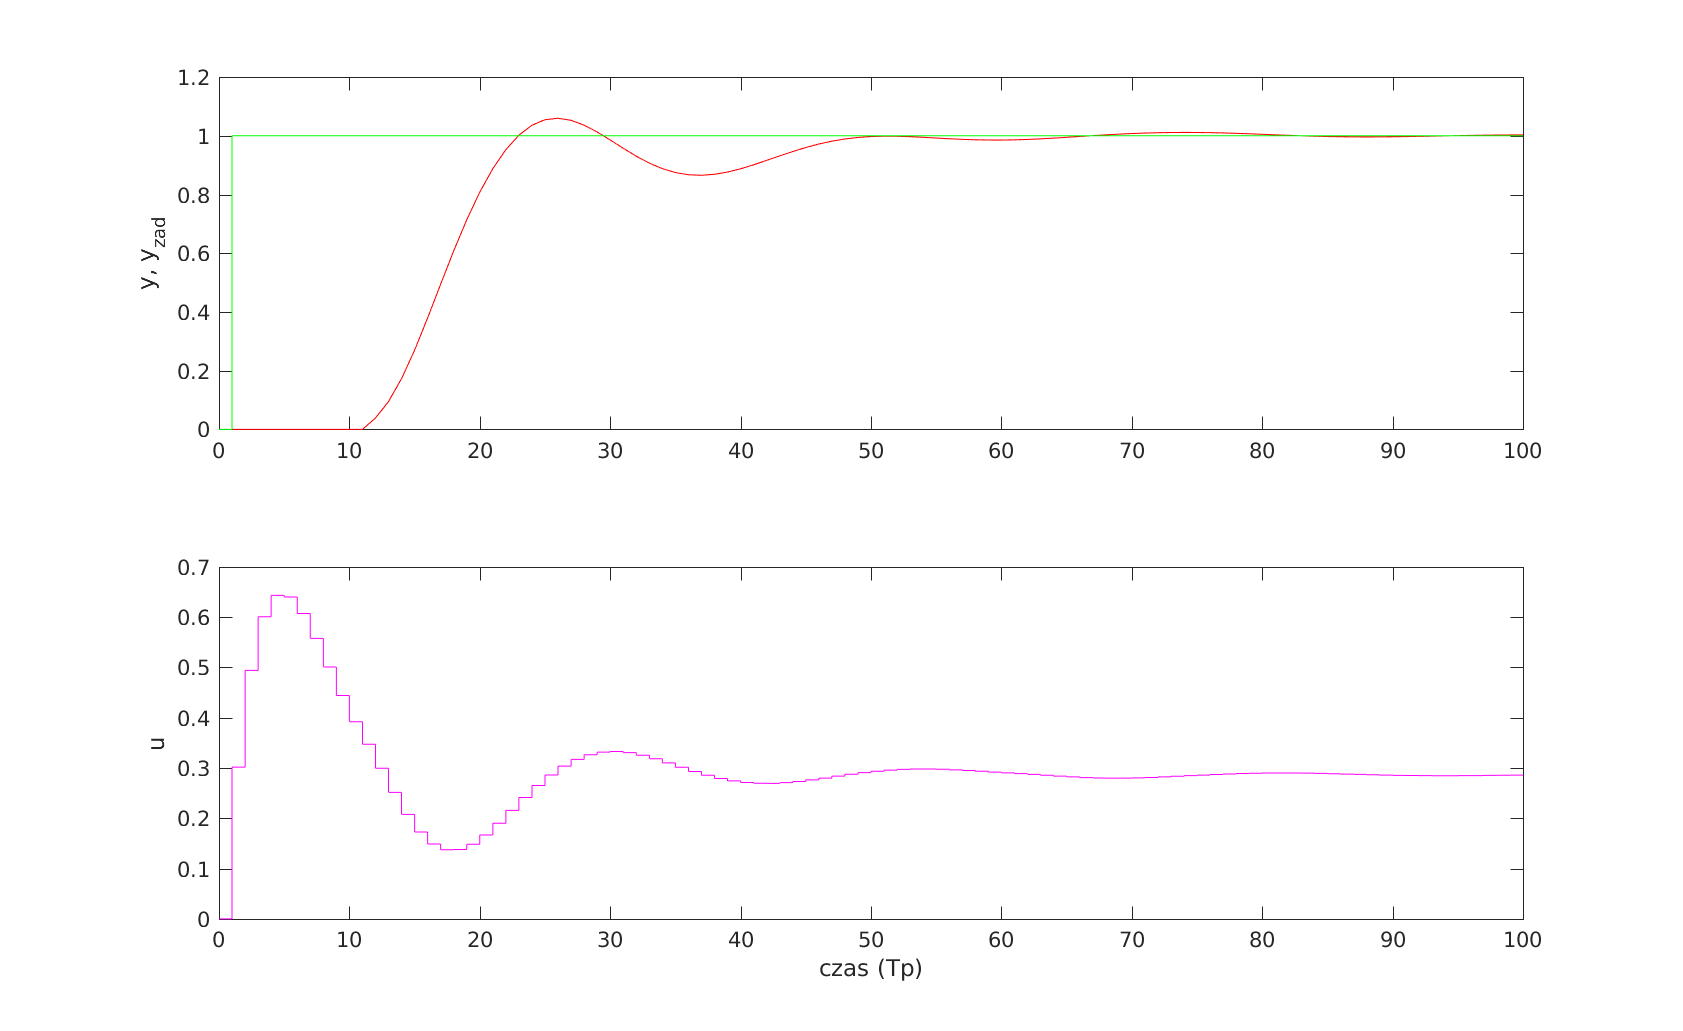
\includegraphics[scale=0.60]{Dostrojony_DmC.png}
\caption{Działanie dostrojonego regulatora DMC}
\end{figure}

\section{Obszary stabilności}
\subsection{Porównanie algorytmów PID i DMC}

\begin{figure}[H]
\centering
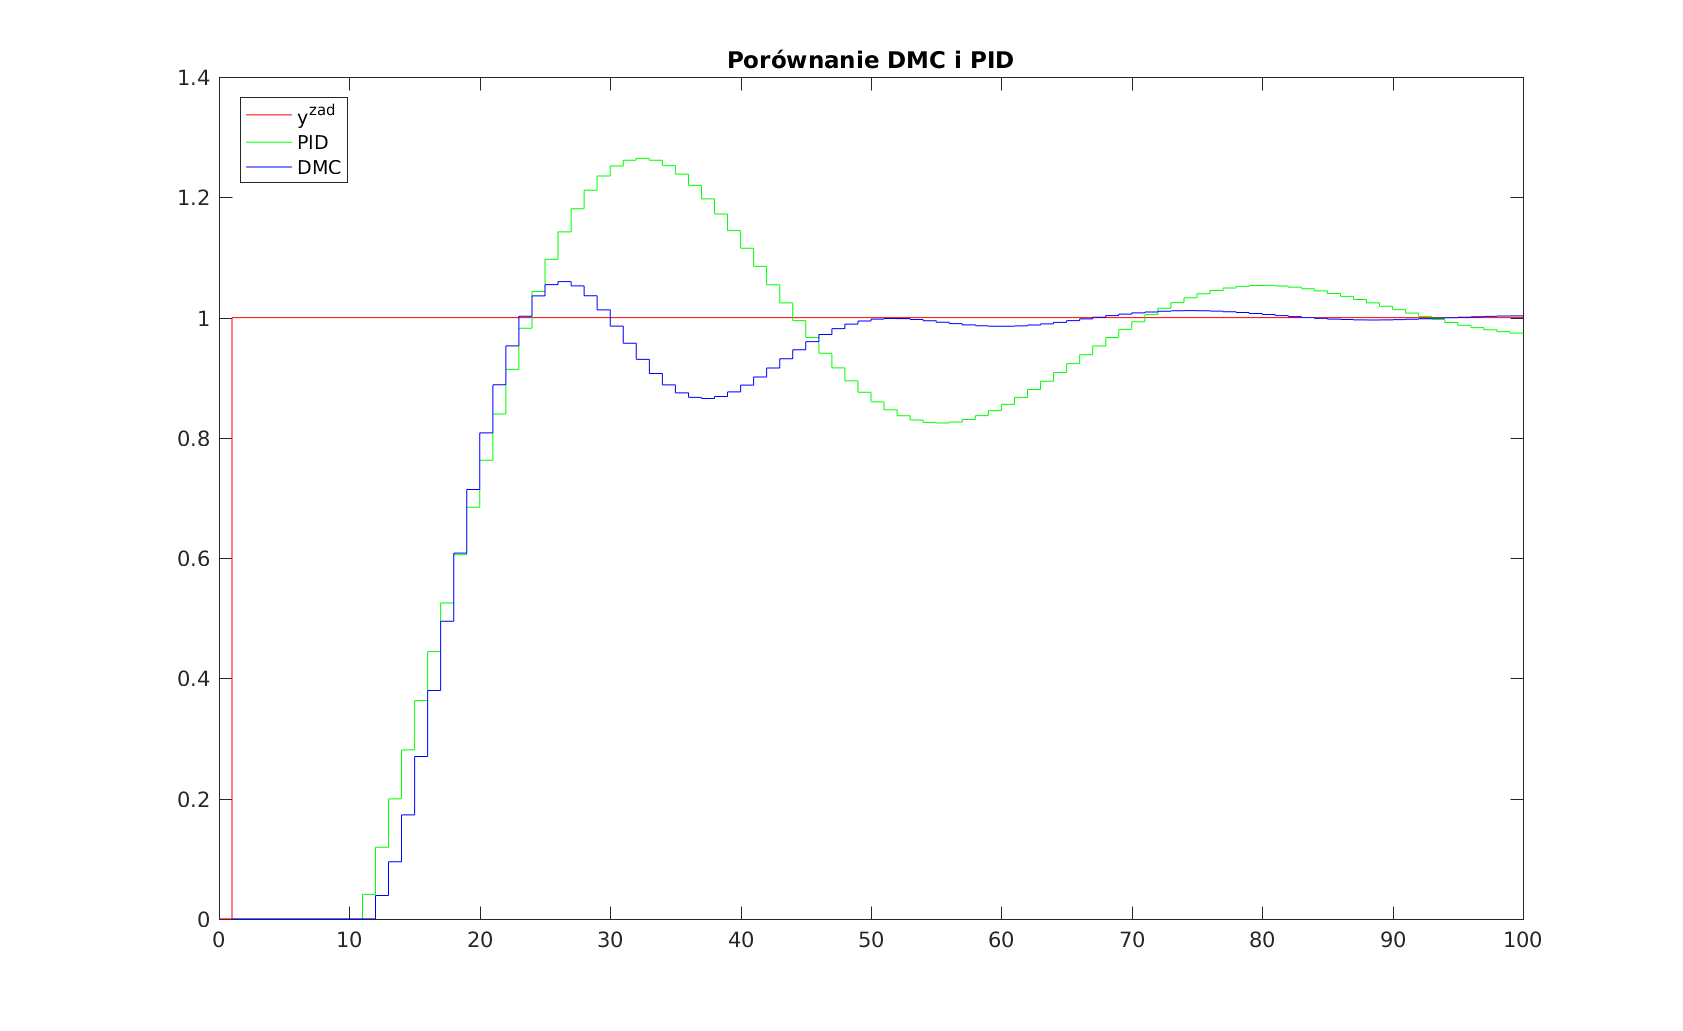
\includegraphics[scale=0.60]{PIDiDMC.png}
\caption{Porównanie PID i DMC}
\end{figure}

Porównując odpowiedzi skokowe obu algorytmów sterowania zauważamy znacznie szybsze osiągnięcie wartości zadanej przez regulator DMC. Biorąc pod uwagę przeregulowanie jak i wartość sygnału sterującego, można z pewnością stwierdzić, że algorytm DMC jest bardziej optymalny dla tego obiektu. 

 
\subsection{Stabilność cyfrowego redulatora PID}
\begin{figure}[H]
\centering
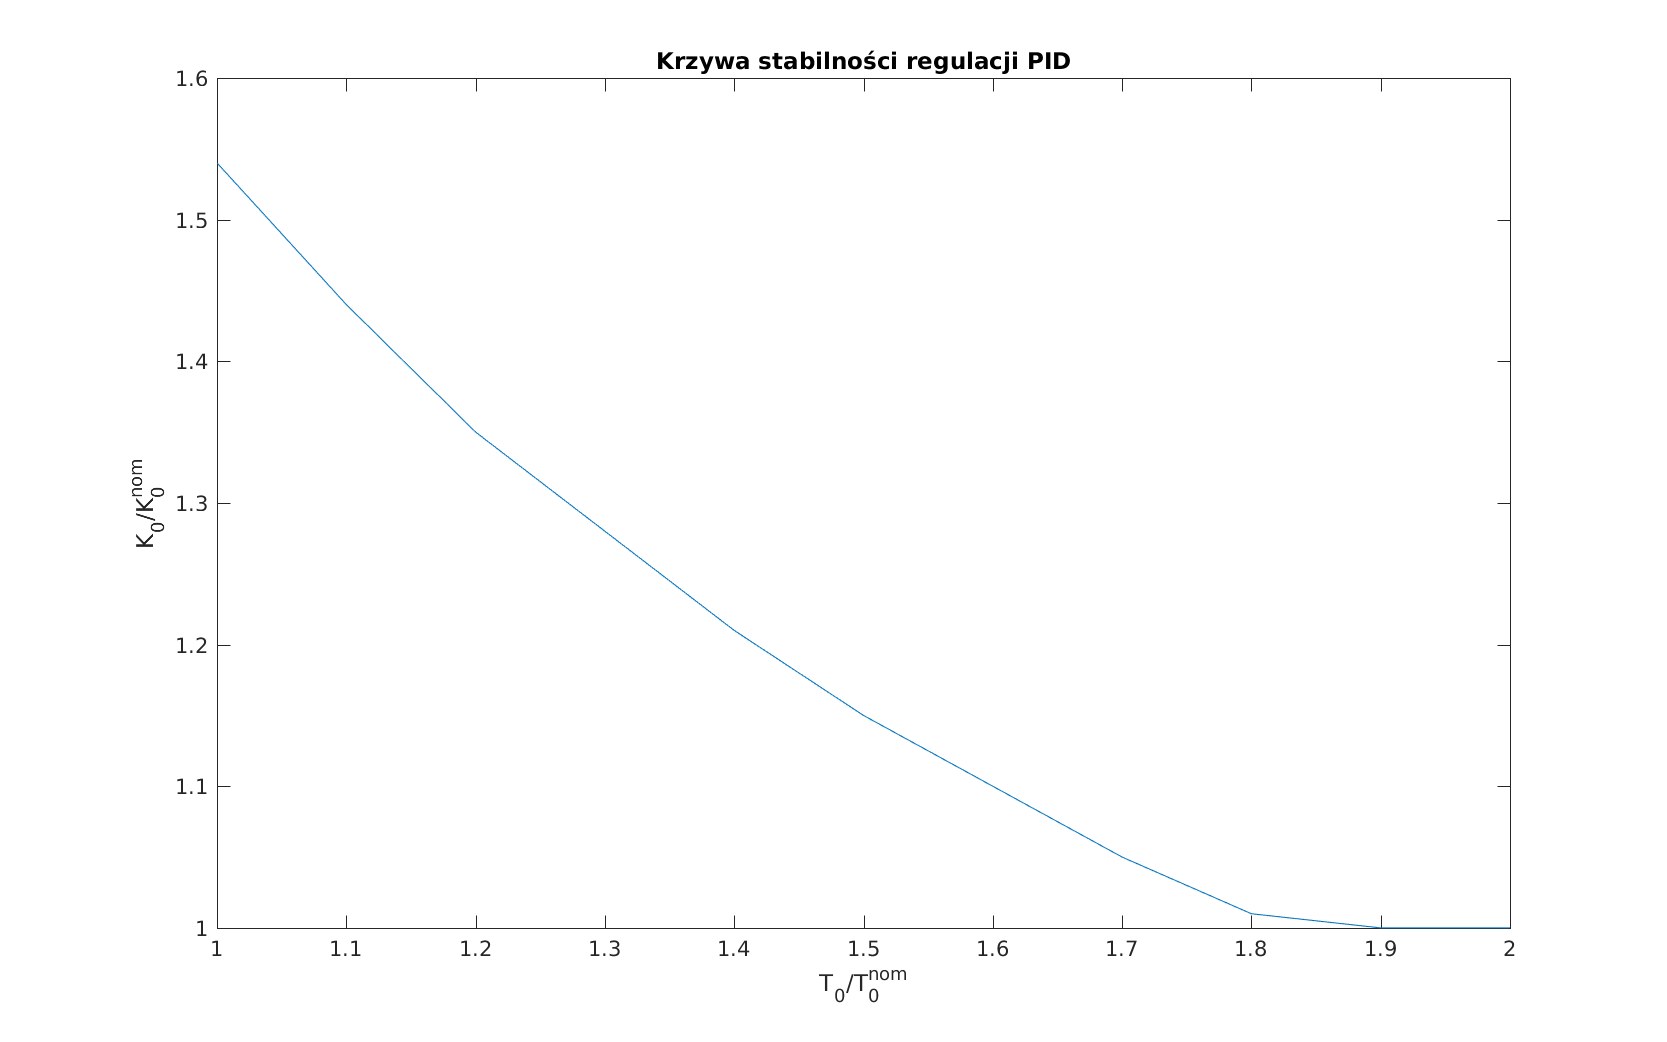
\includegraphics[scale=0.60]{pid_stability.png}
\caption{Obszary stabilności algorytmu PID dla różnych wartości wzmocnienia K i opóźnienia T}
\end{figure}
Wraz ze wzrostem opóźnienia, maleje maksymalne wzmocnienie dla którego układ nie wpada w oscylacje, możliwość zmian parametrów w stosunki do początkowej jest niewielka. Algorytm PID szybko ulega rozregulowaniu nawet dla niewielkich zmian parametrów. 
 
\subsection{Stabilność regulacji DMC}
\begin{figure}[H]
\centering
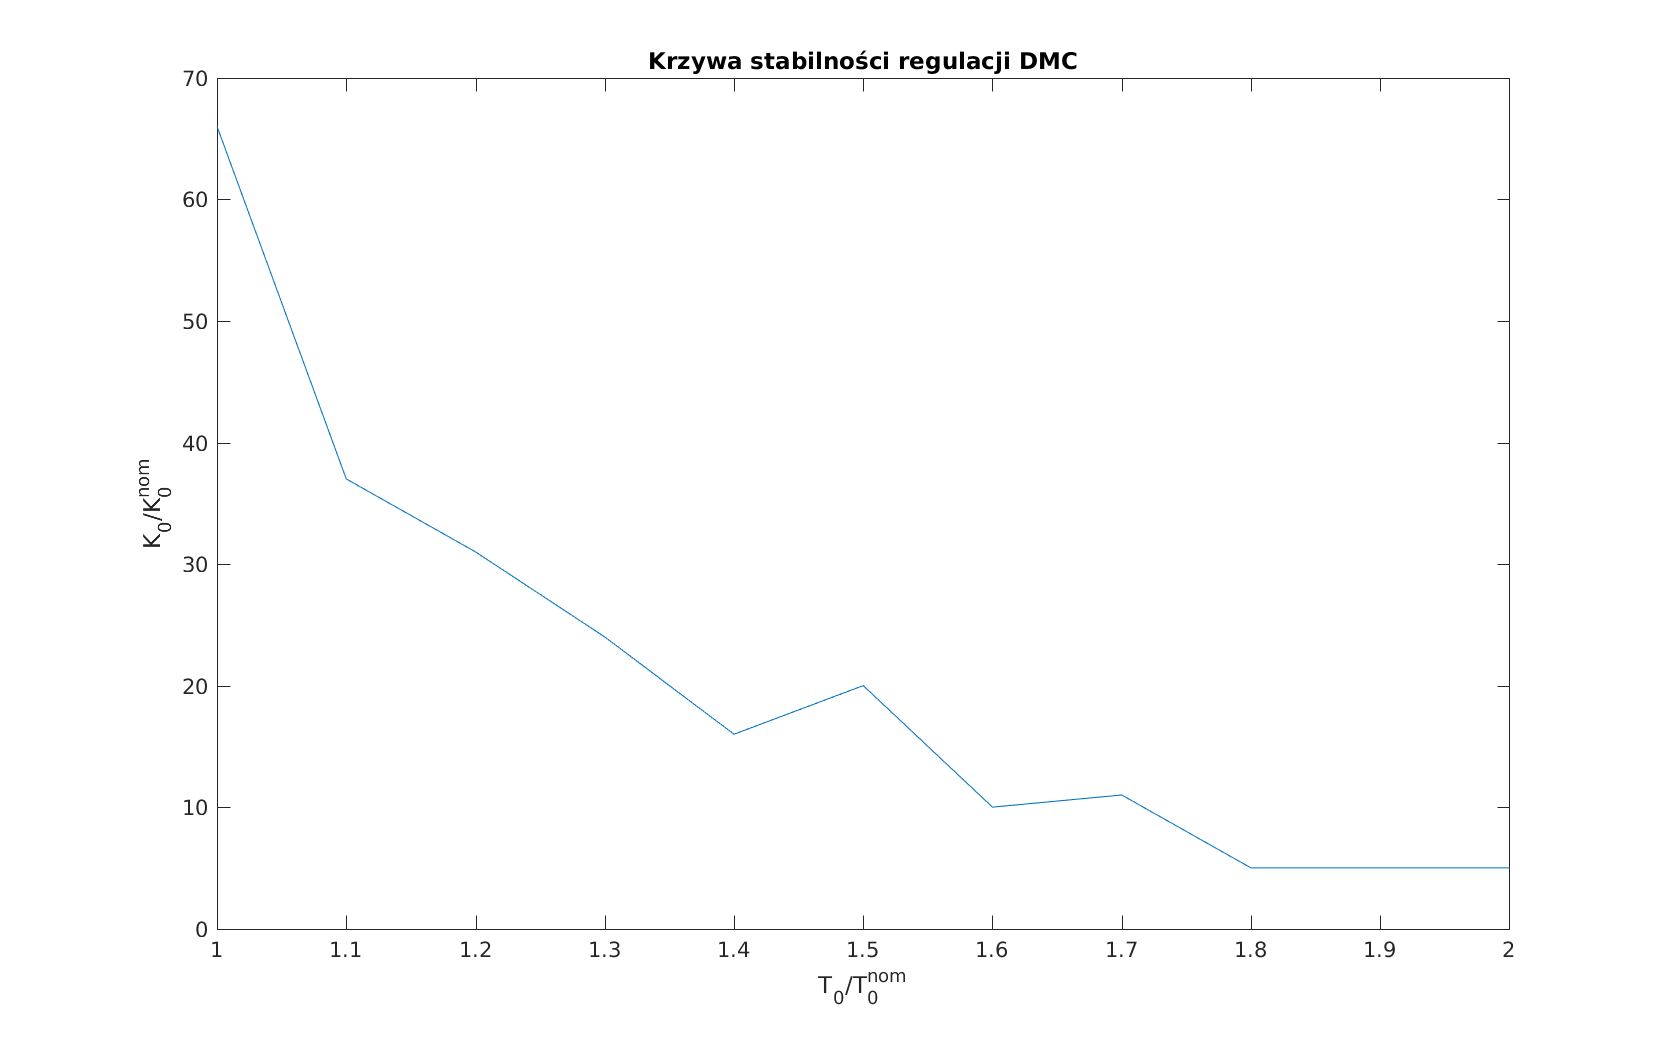
\includegraphics[scale=0.60]{DMC_stability.png}
\caption{Obszary stabilności algorytmu DMC dla różnych wartości wzmocnienia K i opóźnienia T}
\end{figure}

Algorytm DMC jest zdecydowanie bardziej odporny na zmiany parametrów, przy małych zmianach opóźnienia możemy zwiększać wzmocnienie o rzędy wielkości, zachowując szybkość regulacji. Świadczy to o wysokiej stabilności regulacji DMC i sprawia że znajduje on szerokie zastosowanie w sytuacjach, gdzie mamy do czynienia z dynamicznymi zmianami parametrów obiektu. W porównaniu do algorytmu PID, wypada zdecydowanie lepiej. 



 
 

 
 



\end{document}